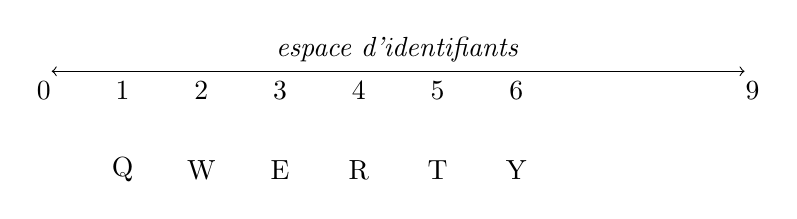
\begin{tikzpicture}[scale=1]

  \draw(-4,1)node{0};

  \draw[<->](-3.9, 1.25)--node[anchor=south]{\textit{espace d'identifiants}} (4.9,1.25);

  \draw(-3,1)node{1};
  \draw(-2,1)node{2};
  \draw(-1,1)node{3};
  \draw(0,1)node{4};
  \draw(1,1)node{5};
  \draw(2,1)node{6};
%  \draw[hide on=1-2,bold on=3](3,1)node{8};
%  \draw[hide on=1-3,bold on=4](4,1)node{8.1};

  \draw(5,1)node{9};

  \draw(-3,0)node{Q};
  \draw(-2,0)node{W};
  \draw(-1,0)node{E};
  \draw(0,0)node{R};
  \draw(1,0)node{T};
  \draw(2,0)node{Y};
%  \draw[hide on=1-2, bold on=3](3,0)node{E};
%  \draw[hide on=1-2, bold on=3](4,0)node{S};


\end{tikzpicture}